\chapter{Tools Selection}
\label{tools-selection}

\section{Top Level Requirements}
The exact implementation of each of the items will be discussed later, but to
simply set our requirements a general list of them is:

\begin{itemlist}
  \item Desktop GUI
  \item Efficient signal processing (for pitch detection)
  \item Real time graph visulization of the signals (osciloscope like)
  \item Access to \textit{libusb} \cite{libusb} API
  \item Access to MIDI API
\end{itemlist}

\section{Language Choice}

\subsection{Java}
The first choice was Java, as it meets all requirements. Desktop GUI can be done
using Swing, a good library for pitch detection is also available (called TasosDSP \cite{TarsosDSP}).
There is also a binding to libusb called usb4java and native MIDI support. \\
Following that idea a functional prototype was built, but a few problems came to rise.
The first is that usb4java high-level API had bugs and was not working correctly.
The solution was to fall back to the lower level API, but that made things much
more complicated as threading and synchronization problems had to be dealt with.
There was no good library for
real time visualization either, which made really hard to both debug and tune the
frequency detection algorithm. On top of that Swing is at least non-pleasant
compared to more modern UI programming, so a second approach came to be.

\subsection{JavaScript}
In alignment with both current work experience and world programming tendencies
JavaScript was taken as a choice. We will see that requirements fit much better now,
for the following reasons. \\
For the desktop GUI, JavaScript has a few nice and mature Desktop GUI frameworks,
like Electron and NW.js. \\
JavaScript is an interpreted language, and for that has a low efficiency when
compared to C++ or Java. That is huge problem, but there is an easy overcome. As
this project tries to build a desktop application, Node.js will be used ultimately,
and it has support for C++ bindings. That means the JavaScript code can call a
compiled C++ library to calculate the pitch, thus solving the problem. \\
Graph visualization should not be a problem either as there are a lot of libraries
for that. \\
The most problematic requirement in Java was \textit{libusb} support. It is available
in JavaScript using \textit{node-usb} \cite{node-usb}, and a few simple tests
returned good results with a much simpler API. MIDI was also tested and worked just fine.

\section{Desktop Framework}
Now that JavaScript is set as our final selection we need an environment to run
it. There are two already listed really mature and popular choices: Electron and NW.js. \\
At first Electron was used to build a test application, because it is the most popular
of the two (in fact even the editor used to write this words is built with it),
but the pitch detection call was running slowly. As a mater of fact it was running
much faster using pure JS code rather than the C++ library. A deeper research
was needed, and the way Electron worked was getting in our way, but first it's
necessary to know what Node.js is.

\subsection{Interpreter}
JavaScript is a interpreted language and thus needs an interpreter. The most
common one is Google V8, which happens to be the same one used in most web
browsers as well as in Node. The difference between browsers and Node is simply
the API that comes with them. Web needs firstly to access the UI (html) and ways to
modify it, it also needs secure and limited access to hardware and internet calls.
Of course that means web JavaScript code cannot use C++ libraries directly. \\
On the other hand Node is a more pure version of V8, it also gives the possibility
to write and call C++ code (feature needed for this project), which ultimately
makes it as capable as any desktop
program can be. Node also comes with a hand-full set of native resources (like
file system and full communication access), but it does \textbf{not} provide
any kind of GUI. Knowing that it is possible to have a better understanding on
how the two desktop environments work.

\subsection{Electron}
Electron by design has at least two processes running \cite{ElectronVsNW},
one for the "web" and other
for Node access. The answer for how the web process access native resources is
also to why the execution of the C++ processing library was slow: it uses
inter-process communication (IPC). IPC makes things a lot slower, which ultimately
makes impossible to use Electron in this project.

\subsection{Node Webkit}
Differently from Electron, NW.js \cite{NWjs, ElectronVsNW} takes the Node environment
and combines it with Chromium into a single process, removing the use of IPC.
Initial tests reported that the pitch detection library has fast
execution as expected.

\section{Architectural Tools}
NW.js will go only as far as to give access to both Node and DOM API's. But that
is too crude, and not what we wanted by given up on Java Swing. Again based on
current work experience and world tendencies the setup chosen is React + Redux. \\
React \cite{React} is a library created by Facebook and world wide used for UI applications.
It uses a declarative component-based system that makes it easy to build scalable
and reusable code.\\
React only go as far to help building the UI, but we also need to pass the state
of the application to the UI components, and that is where Redux comes in. It
keeps all the application state stored in a single place, described by transition
functions. That makes the storage system easy to be tested and used, because all
actions (that modify the state) must be well defined and it doesn't rely on the
UI (React), making it easy to test.\\
\autoref{react-redux-diagram} shows the flow of an application that uses
React + Redux. It is obvious to see the simplicity it has, a single path must be followed.
This simplicity is what makes it much easier to use against other frameworks like
Java Swing.

\begin{figure}[htb]
	\caption{React Redux Flow Diagram}
  \label{react-redux-diagram}
	\begin{center}
    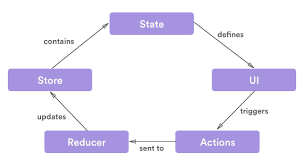
\includegraphics[scale=1]{images/react-redux-diagram.png}
	\end{center}
  \legend{Source: \citeonline{react-redux-diagram-source}}
\end{figure}

\section{Fast Signal Processing}
Pitch detection is a heavy problem to solve, and good implementations are time
consuming, so we need efficiency to run it real-time. The library already said
to be used didn't actually existed, the only one available was a pure JavaScript
library \cite{pitchfinder} which is not suitable for this project. The solution
was to build our own library based on both the pure JavaScript one and TarsosDSP
\cite{TarsosDSP}. Implementation details discussed further on \autoref{pitch-detection}.

\section{Real Time Visualization}
There are lots of charting libraries available for use with web interfaces (and
by extension NW.js), unfortunately none was good fit for real time high density
signals such as audio. The solution was again to build one, since all other things
are looking to run smoothly in JavaScript, implementation details on TODO-REF.
